\documentclass[aspectratio=1610, professionalfonts, 10pt]{beamer}

% Lade das TU Dortund Theme von Max Nöthe
\usefonttheme[onlymath]{serif}
\usetheme[showtotalframes]{tudo}

% Lade richtiges Sprachpaket
\ifluatex
    \usepackage{polyglossia}
    \setmainlanguage{english}
\else
    \ifxetex
        \usepackage{polyglossia}
        \setmainlanguage{german}
    \else
        \usepackage[german]{babel}
    \fi
\fi

% Lade wichtige Mathematikpakete
\usepackage{amsmath}
\usepackage{amssymb}
\usepackage{mathtools}
\usepackage{cancel}
\usepackage[
  locale=DE,                   % deutsche Einstellungen
  separate-uncertainty=true,   % Immer Fehler mit \pm
  per-mode=symbol-or-fraction, % m/s im Text, sonst Brüche
]{siunitx}
\usepackage[absolute,overlay]{textpos}
\usepackage{framed}
\usepackage{multicol}
\usepackage{setspace}
\usepackage{graphicx}
\usepackage{booktabs}
\usepackage{caption}
\usepackage{appendixnumberbeamer}
\usepackage{tikz}
\usepackage[export]{adjustbox}
\usepackage{color}
\usepackage{multirow}
\usepackage{subfigure}
\usepackage{listings}

\definecolor{dkgreen}{rgb}{0,0.6,0}
\definecolor{gray}{rgb}{0.5,0.5,0.5}
\definecolor{mauve}{rgb}{0.58,0,0.82}

\lstset{frame=tb,
  language=bash,
  aboveskip=3mm,
  belowskip=3mm,
  showstringspaces=false,
  columns=flexible,
  basicstyle={\small\ttfamily},
  numbers=none,
  numberstyle=\tiny\color{gray},
  keywordstyle=\color{blue},
  commentstyle=\color{dkgreen},
  stringstyle=\color{mauve},
  breaklines=true,
  breakatwhitespace=true,
  tabsize=3
}


% Lade Paket zur Nutzung von Schleifen
\usepackage{forloop}

% ------------------------- Präsentationsinformationen -------------------------

% Titel:
\title{\textbf{LiDO3: \\ The Linux Dortmund cluster}}
% Autoren:
\author[Kevin Sedlaczek, Björn Wendland]{\textit{Kevin Sedlaczek, Björn Wendland}}
% Titelbild:
% \titlegraphic{\includegraphics[width=0.22\linewidth, rotate=270]{fig/title.png}}

% Datum:
\date{\today}
% Lehrstuhl/Fakultät:
\institute[TU Dortmund]{Lehrstuhl für Experimentelle Physik IV}

\institute[%
  {exp. physik 4}
  % {\includegraphics[height=\headerheight]{logos/fact.pdf}}%
  % \hspace{1em}%
  % {\includegraphics[height=\headerheight]{logos/e5logo.pdf}}%
]{
  {
\includegraphics[height=1.0cm]{logos/tu.pdf}}%
  % \hspace{1em}%
  % {\includegraphics[height=0.75cm]{logos/ethz.pdf}}%
  % \hspace{1em}%
  % {\includegraphics[height=0.75cm]{logos/isdc.pdf}}%
  % \hspace{1em}%
  % {\includegraphics[height=0.75cm]{logos/uniwue.pdf}}%
}

\AtBeginSection[]{
  \begin{frame}
  \vfill
  \centering
  \begin{beamercolorbox}[sep=8pt,center,shadow=true]{title}
    \usebeamerfont{title}\insertsectionhead\par%
  \end{beamercolorbox}
  \vfill
  \end{frame}
}
% Titelgrafik:
% \titlegraphic{\includegraphics[width=0.4\textwidth]{logos/FACTLogo_preliminary.png}\hfill\includegraphics[width=0.4\textwidth]{logos/e5logo_green_text.pdf}}


\makeatletter
    \newenvironment{withoutheadline}{
        \setbeamertemplate{headline}[default]
        \def\beamer@entrycode{\vspace*{-\headheight}}
    }{}
\makeatother

\begin{document}
{
\setbeamertemplate{headline}{}
\maketitle
}

\begin{frame}[t]{Inhalt}
  \begin{enumerate}
    \item Aufbau und Funktion
    \item Technische Daten
    \item Zugang
    \item Personal Space
    \item Scheduling und Starten von Jobs
    \item SLURM jobs
    \item SLURM Skripte
    \item Software auf LiDO
    \item Literatur
  \end{enumerate}
\end{frame}

\begin{frame}{Linux Cluster Dortmund (3. Generation)}
  \underline{\textbf{Technische Daten:}}
  \begin{itemize}
    \item Offiziell in Betrieb seit Beginn 2018
    \item Verschiedene Rechenknoten (insg. 366 Knoten / 8160 CPU cores (Intel Xeon))
    \item 40 GPU Beschleuniger NvidiaTesla K40
    \item Mehr als 30\,TB RAM, mind. 64\,GB /  Knoten
    \item Paralleles Dateisystem mit 1,28\,PB (sichtbar von jedem Knoten)
    \item Pro Knoten mind. 2\,TB lokaler Speicher
    \item QDR(40\,Gbit/s) Netzwerkanbindnug
    \item Queueing system \textbf{SLURM}
    \item 2 Gateway server
    \item Modulares Software system mit vielen bereits installierten Anwendungen (Compiler, Profiler, Debugger, Scientific software, ...)
  \end{itemize}
\end{frame}

\begin{frame}{Zugangsantrag}
  Um Zugang zu LiDO3 zu erhalten muss lediglich online ein Antrag gestellt werden.
  \begin{columns}
    \begin{column}{0.475\textwidth}
      \centering
      
\includegraphics[width=\textwidth]{figs/lido_web.png}
    \end{column}
    \begin{column}{0.475\textwidth}
      \centering
      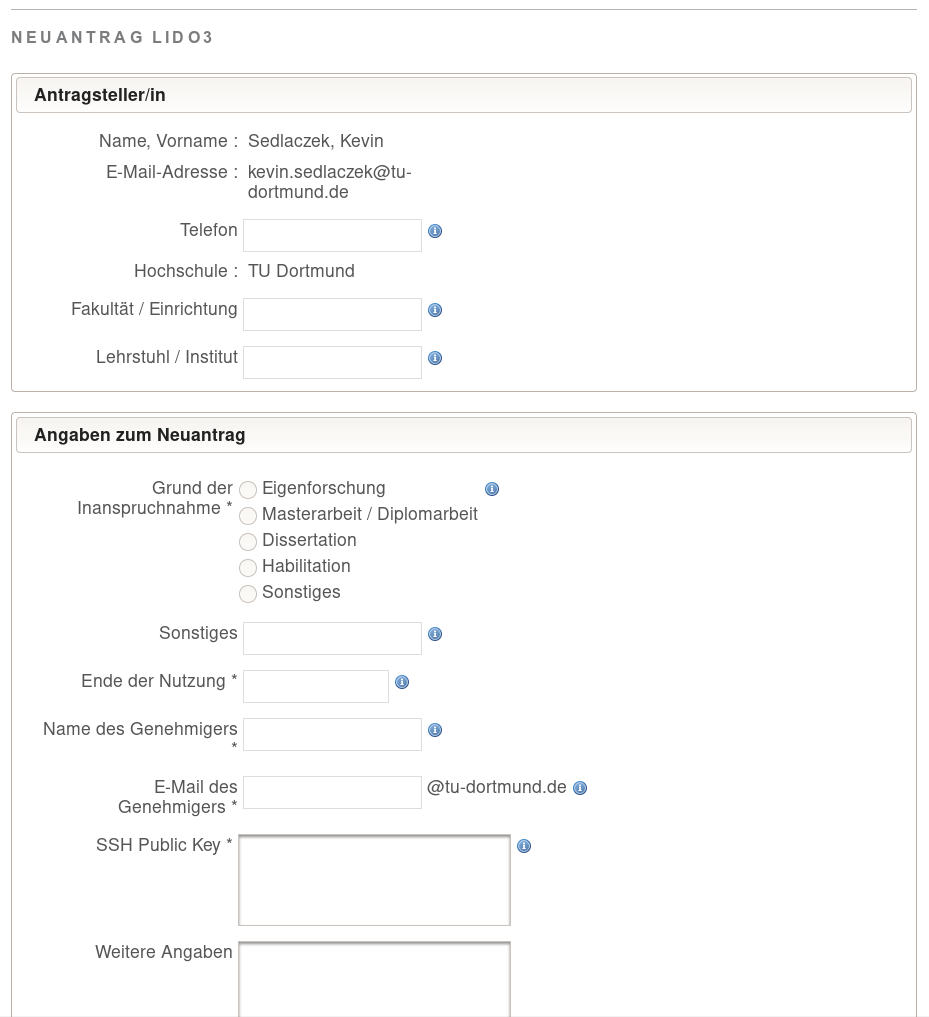
\includegraphics[width=0.8\textwidth]{figs/Neuantrag.png}
    \end{column}
  \end{columns}
\end{frame}

\begin{frame}{Zugang per SSH über die gateways}
  \begin{columns}
    \begin{column}{0.475\textwidth}
      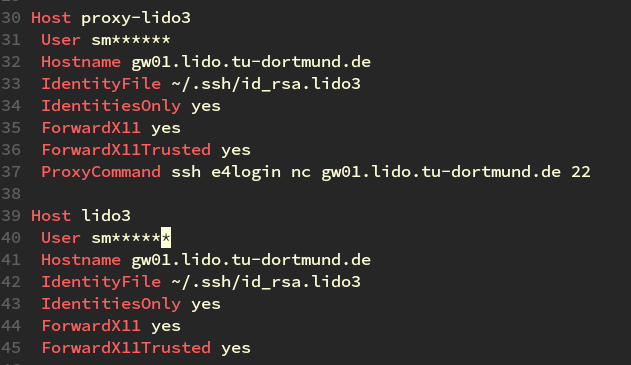
\includegraphics[width=\textwidth]{figs/ssh_conf.png}
    \end{column}
    \begin{column}{0.475\textwidth}
      \begin{itemize}
        \item 2 gateways zur Wahl: \texttt{gw01.lido.tu-dortmund.de} \texttt{gw02.lido.tu-dortmund.de}
        \item von außerhalb des Uni Netzes über proxy via \texttt{login.e4.physik.tu-dortmund.de}
      \end{itemize}
    \end{column}
  \end{columns}
\end{frame}

\begin{frame}{Personal Space}
  \texttt{/home/<username>}
  \begin{itemize}
    \item Insgesamt 14\,TB Speicher für home Verzeichnisse
    \item Jeder user hat 32\,GB Speicher (max. 100\,000 Dateien) unter \texttt{/home/<username>}
    \item Das home-Verzeichnis wird regelmäßig gesichert
  \end{itemize}
  \texttt{/work/<username>}
  \begin{itemize}
    \item Insgesamt 1280\,TB zentrales paralleles Dateisystem (work Verzeichnisse)
    \item Jeder user hat 1\,TB work Speicher unter \texttt{/work/<username>}
    \item ACHTUNG: work Speicher wird \textbf{nicht} gesichert: Datenverlust möglich \rightarrow nur reproduzierbare Dateien hier speichern oder extern sichern!
  \end{itemize}
  Die home-Partitionen \texttt{/home/<username>} sind auf Rechennodes nur \textbf{read-only} gemountet!
\end{frame}

\begin{frame}{Best practice}
  BeeGFS Dateisystem nicht gut geeignet für viele zeitintensive Dateioperationen, daher Nutzung des lokalen \texttt{/scratch} Ordners.
  \begin{itemize}
    \item \texttt{/scratch} existiert mit mind. 2\,TB auf jedem Knoten, allerdings nur lokal
  \end{itemize}
  \begin{enumerate}
    \item Bei Jobstart jeweils Daten von \texttt{/home} nach \texttt{/scratch} kopieren
    \item Daten werden in \texttt{/scratch} verarbeitet
    \item Nach Durchführung des jobs von \texttt{/scratch} zurück nach \texttt{/work} kopieren
    \item Evtl. wichtige Ergebnisse in \texttt{/home} sichern
  \end{enumerate}
  Zum Bearbeiten von Dateien lassen sich die Partitionen einzeln via \texttt{sshfs} oder \texttt{sfp} lokal mounten. Natürlich stehen auch tools wie \texttt{scp} zur Verfügung und auf lido eine bash, sowie z.B. MidnightCommander (\texttt{mc}).

\end{frame}

\begin{frame}{Scheduling}
  \begin{itemize}
    \item Jobs werden durch Schedulingsystem SLURM priorisiert
    \item Mögliche Partitionen:
  \end{itemize}
  \begin{table}
    \begin{tabular}{l
                    c
                    }
            \toprule
            Partition & Max. walltime \\
            \midrule
            short & 02:00:00 \\
            med & 08:00:00 \\
            long & 48:00:00 \\
            ultralong & 672:00:00 \\
            \bottomrule
    \end{tabular}
    \caption{Available public partitions.}
    \label{tab:part}
  \end{table}
\end{frame}

\begin{frame}{Spezifikation der benötigten Knoten}
  Zunächst interaktiv vom gateway:
  \begin{itemize}
    \item Reservieren eines Knotens mit Hilfe von \texttt{salloc}
    \item \texttt{salloc -N x -C F -c c --mem=y -t w -p part}
    \item Dabei werden x Knoten mit Feature F angefordert. Man benötigt höchtens c Cores, y MB pro Knoten an RAM und w=hh:mm:ss an Walltime. Die Anforderung wird der Partition part zugeordnet.
    \item Starten einer bash Konsole auf dem allokierten Knoten (nach evtl. Queueing time):
    \item \texttt{srun --pty bash}
  \end{itemize}
\end{frame}

\begin{frame}{SLURM-jobs}
  \begin{itemize}
    \item Jeder SLURM-job besitzt eine Job ID
    \item Anzeigen des Status' aller submitteten jobs via \texttt{squeue -u <username>}
    \item Löschen/Abbrechen eines jobs via \texttt{scancel ID}
    \item Anzeigen der erwarteten Startzeit eines jobs \texttt{squeue --start -j ID}
    \item Grafische Übersicht via \texttt{sview}
  \end{itemize}
\end{frame}

\begin{frame}{SLURM Skript}
  \begin{itemize}
    \item Bequemes Spezifizieren und Starten von jobs
    \item Verschiedene Eigenschaften können spezifiziert werden:
    \begin{itemize}
      \item Walltime
      \item Partition
      \item Speicher
      \item Prozesse pro Knoten
      \item Knoteneigenschaft
      \item Email Benachrichtigungen
      \item Spezielle Ausgabedatei
      \item Programmaufruf
      \item Laden von software
    \end{itemize}
  \end{itemize}
\end{frame}

\begin{frame}{SLURM Skript}
  \centering
  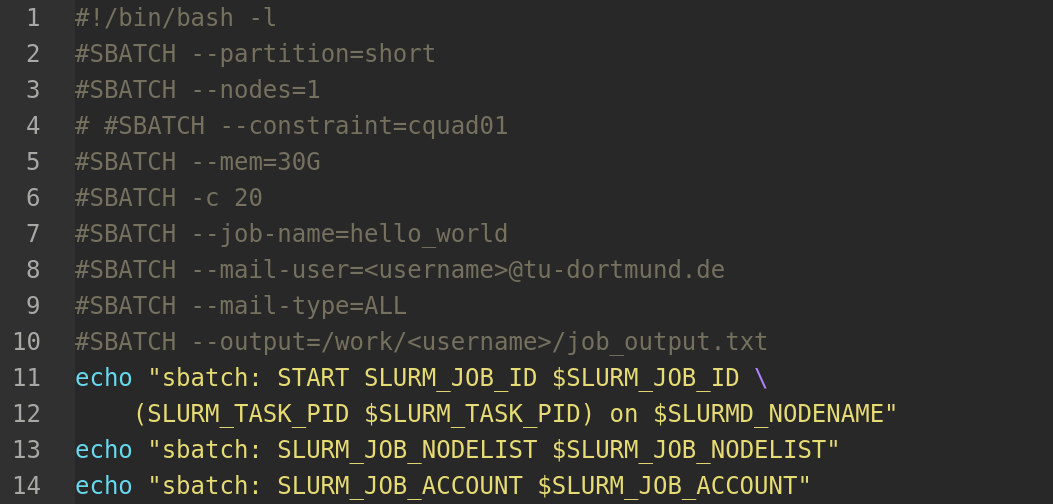
\includegraphics[width=0.8\textwidth]{figs/slurm_oben.png}
\end{frame}

\begin{frame}{SLURM Skript}
  \centering
  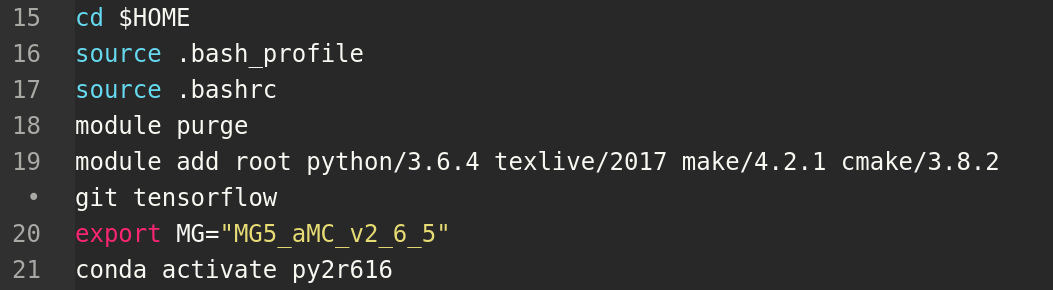
\includegraphics[width=0.8\textwidth]{figs/slurm_software.png}
\end{frame}

\begin{frame}{SLURM Skript}
  \centering
  
\includegraphics[width=0.8\textwidth]{figs/slurm_end.png}
\end{frame}

\begin{frame}{Module}
  \begin{itemize}
    \item Software, die für Entwicklung und Ausführung benötigt wird, wird in Module organisiert
    \item Ermöglicht saubere Umgebungen, konkurrierende software, richtige Versionen
    \item Mit \texttt{module list} werden aktuell geladene Module angezeigt
    \item mit \texttt{module avail} erscheint eine Liste verfügbarer Module
    \item \texttt{module add module\_name} lädt das Modul \texttt{module\_name}
    \item \texttt{module rm module\_name} entfernt das Modul \texttt{module\_name}
    \item \texttt{module purge} entlädt alle geladenen Module
  \end{itemize}
  Siehe dazu auch \url{https://www.lido.tu-dortmund.de/cms/de/LiDO3/Software/index.html}
\end{frame}

\begin{frame}{Lokale software}
  \begin{itemize}
    \item \texttt{conda} oder \texttt{miniconda} im home-Verzeichnis installieren und Installation mit \texttt{--user}
    \item Software im home-Verzeichnis, außer wenn Schreibrechte nötig sind (z.B. MG5)
  \end{itemize}

\end{frame}

\begin{frame}{Literatur}
  \begin{itemize}
    \item \url{https://www.lido.tu-dortmund.de/cms/de/LiDO3/lido3kurz.pdf}
    \item \url{https://www.lido.tu-dortmund.de/cms/de/LiDO3/Software/index.html}
    \item \url{https://service.tu-dortmund.de/group/intra/lido3neuantrag}
    \item \url{https://github.com/KevSed/LiDO-howto/tree/master/talk}
  \end{itemize}
\end{frame}


\end{document}
